\section{The GlueX Experiment}\label{sec:the-gluex-experiment}
GlueX, short for the Gluonic Excitation experiment located at the Thomas Jefferson National Accelerator Facility (JLab), first began collecting publication-quality data in 2016 with the goal of establishing the spectrum of light mesonic states including hybrid mesons and glueballs.

\begin{figure}
  \begin{center}
    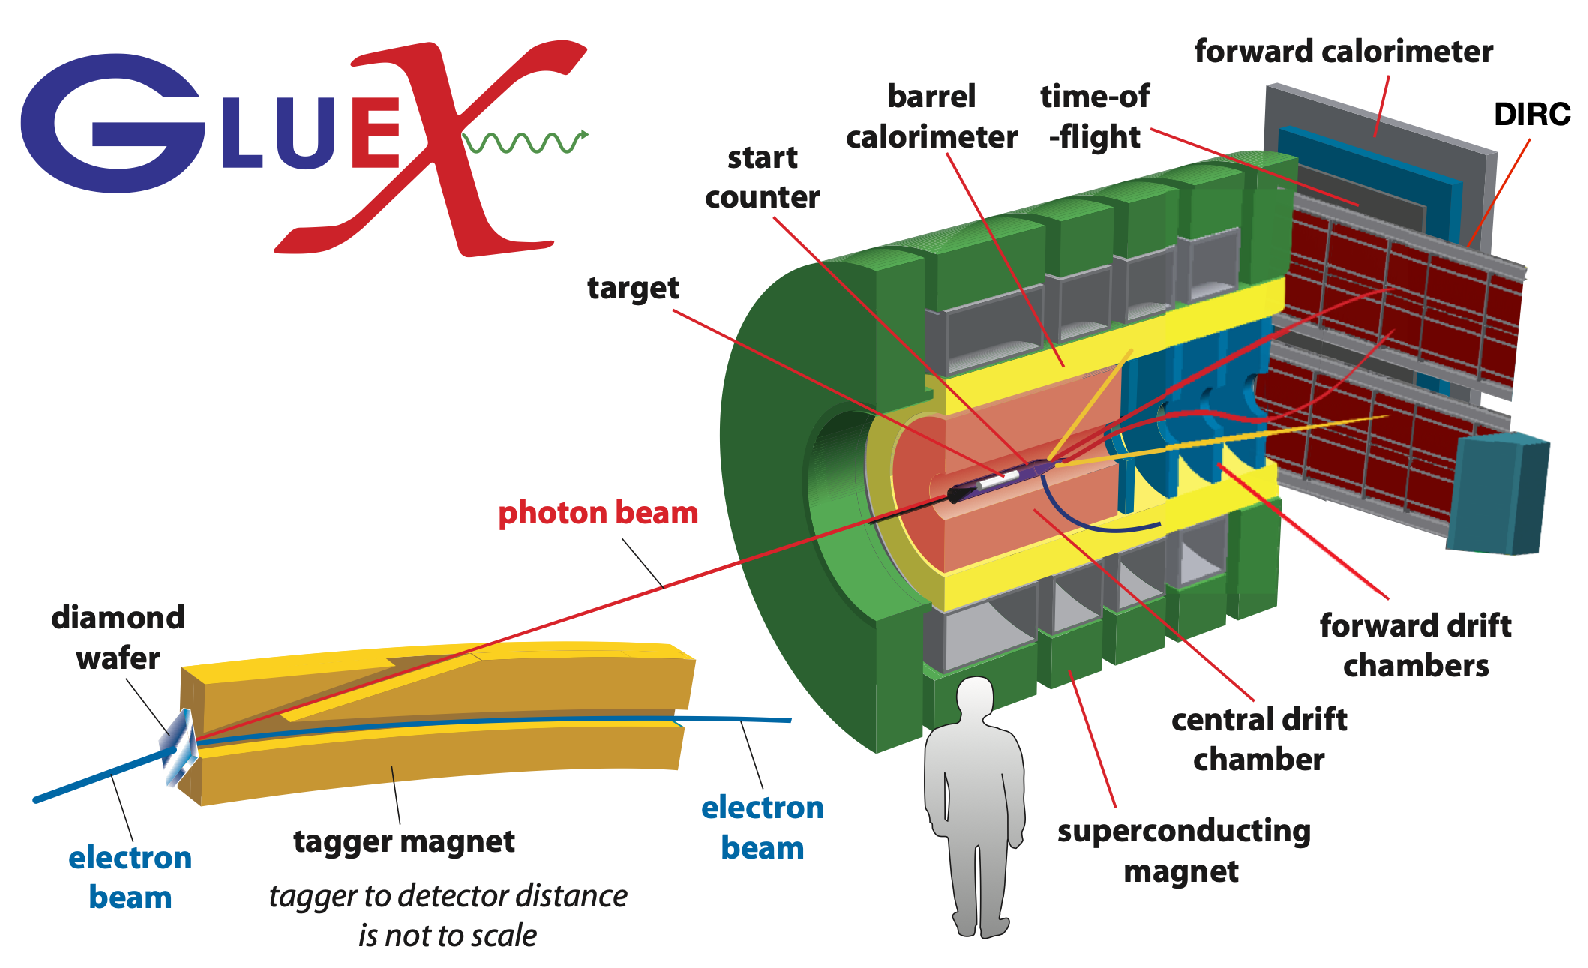
\includegraphics[width=0.8\textwidth]{figures/gluex_detector.png}
  \end{center}
  \caption{A diagram of the GlueX detector at JLab. The DIRC detector was installed in 2019 and was only present for about half of the data analyzed in this study.{\color{red}CITE}}\label{fig:gluex-detector}
\end{figure}

GlueX receives an unpolarized electron beam from the Continuous Electron Beam Accelerator Facility (CEBAF), which is then converted to linearly polarized photons via coherent bremsstrahlung from a diamond radiator (see \Cref{fig:gluex-detector}). The scattering electrons are detected in an array of high-resolution scintillators called the Tagger Microscope (TAGM) which covers beam energies between $8$ and $\SI{9}{\giga\eV}$, a region of energy referred to as the ``coherent peak''. The orientation of the diamond radiator is optimized to produce the highest photon polarization and flux in this region (see \Cref{fig:gluex-polarization}). The rest of the energy range, regions from about $3$--$\SI{8}{\giga\eV}$ and $9$--$\SI{12}{\giga\eV}$, are covered by the lower-resolution Tagger Hodoscope (TAGH). These elements are used to determine only the photon energy, which is equal to the difference between the incident and outgoing electron energies~\cite{adhikari_gluex_2021}.


\begin{figure}
  \begin{center}
    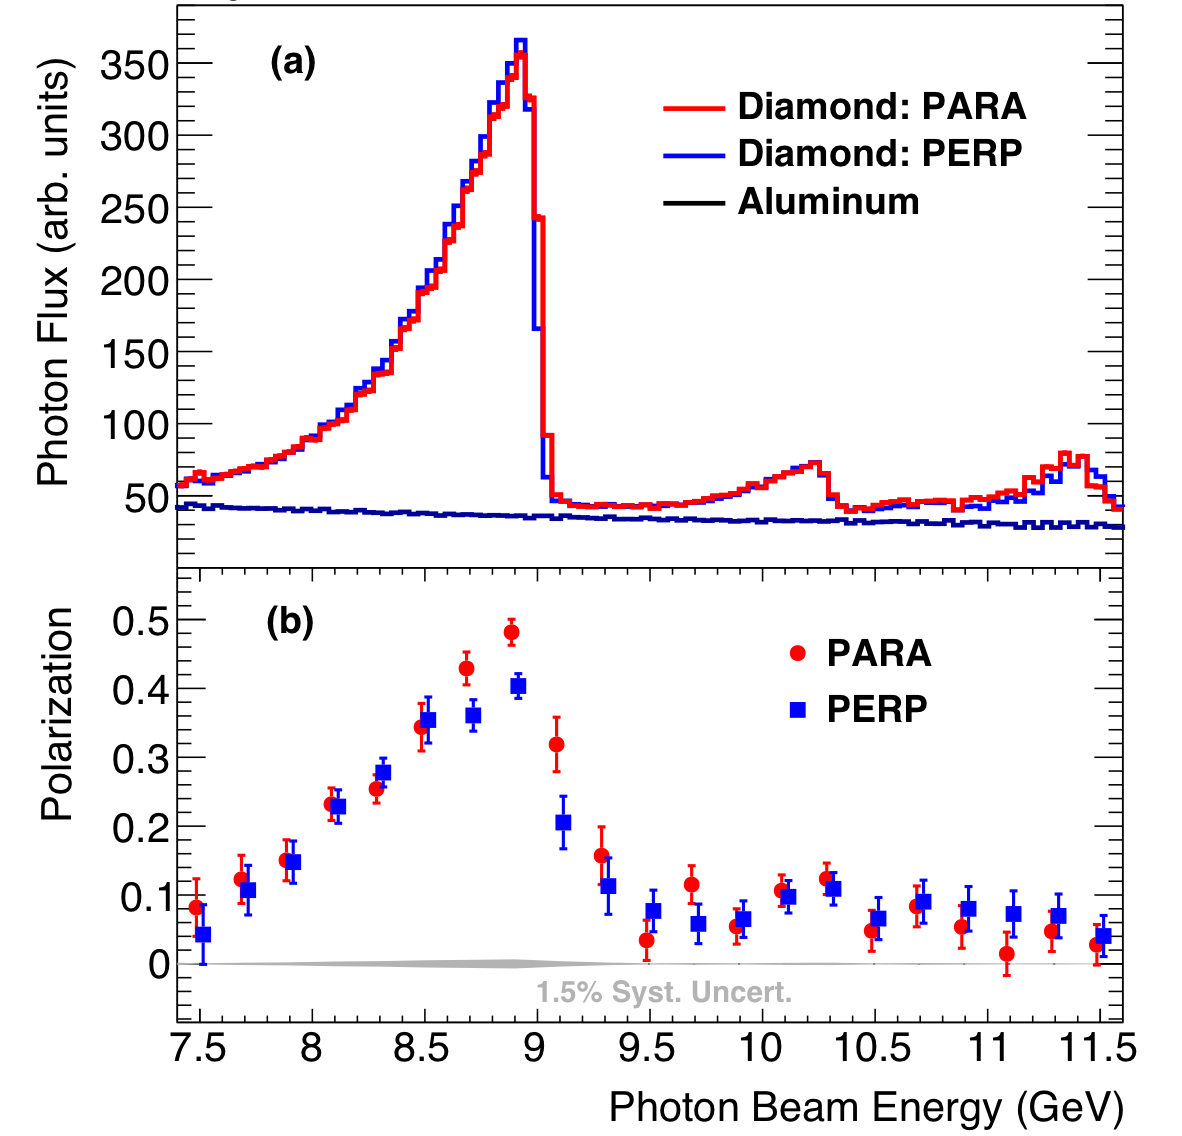
\includegraphics[width=0.95\textwidth]{figures/gluex_polarization.png}
  \end{center}
  \caption{(a) Collimated photon beam intensity versus energy as measured by the Pair Spectrometer. (b) Collimated photon beam polarization as a function of beam energy, as measured by the Triplet Polarimeter, with data points offset horizontally by $\pm\SI{0.015}{\giga\eV}$ for clarity. The labels PARA and PERP refer to orientations of the diamond radiator that result in polarization planes that are parallel and perpendicular to the horizontal, respectively (figure and caption from \cite{adhikari_gluex_2021}).}\label{fig:gluex-polarization}
\end{figure}


\begin{figure}
  \begin{center}
    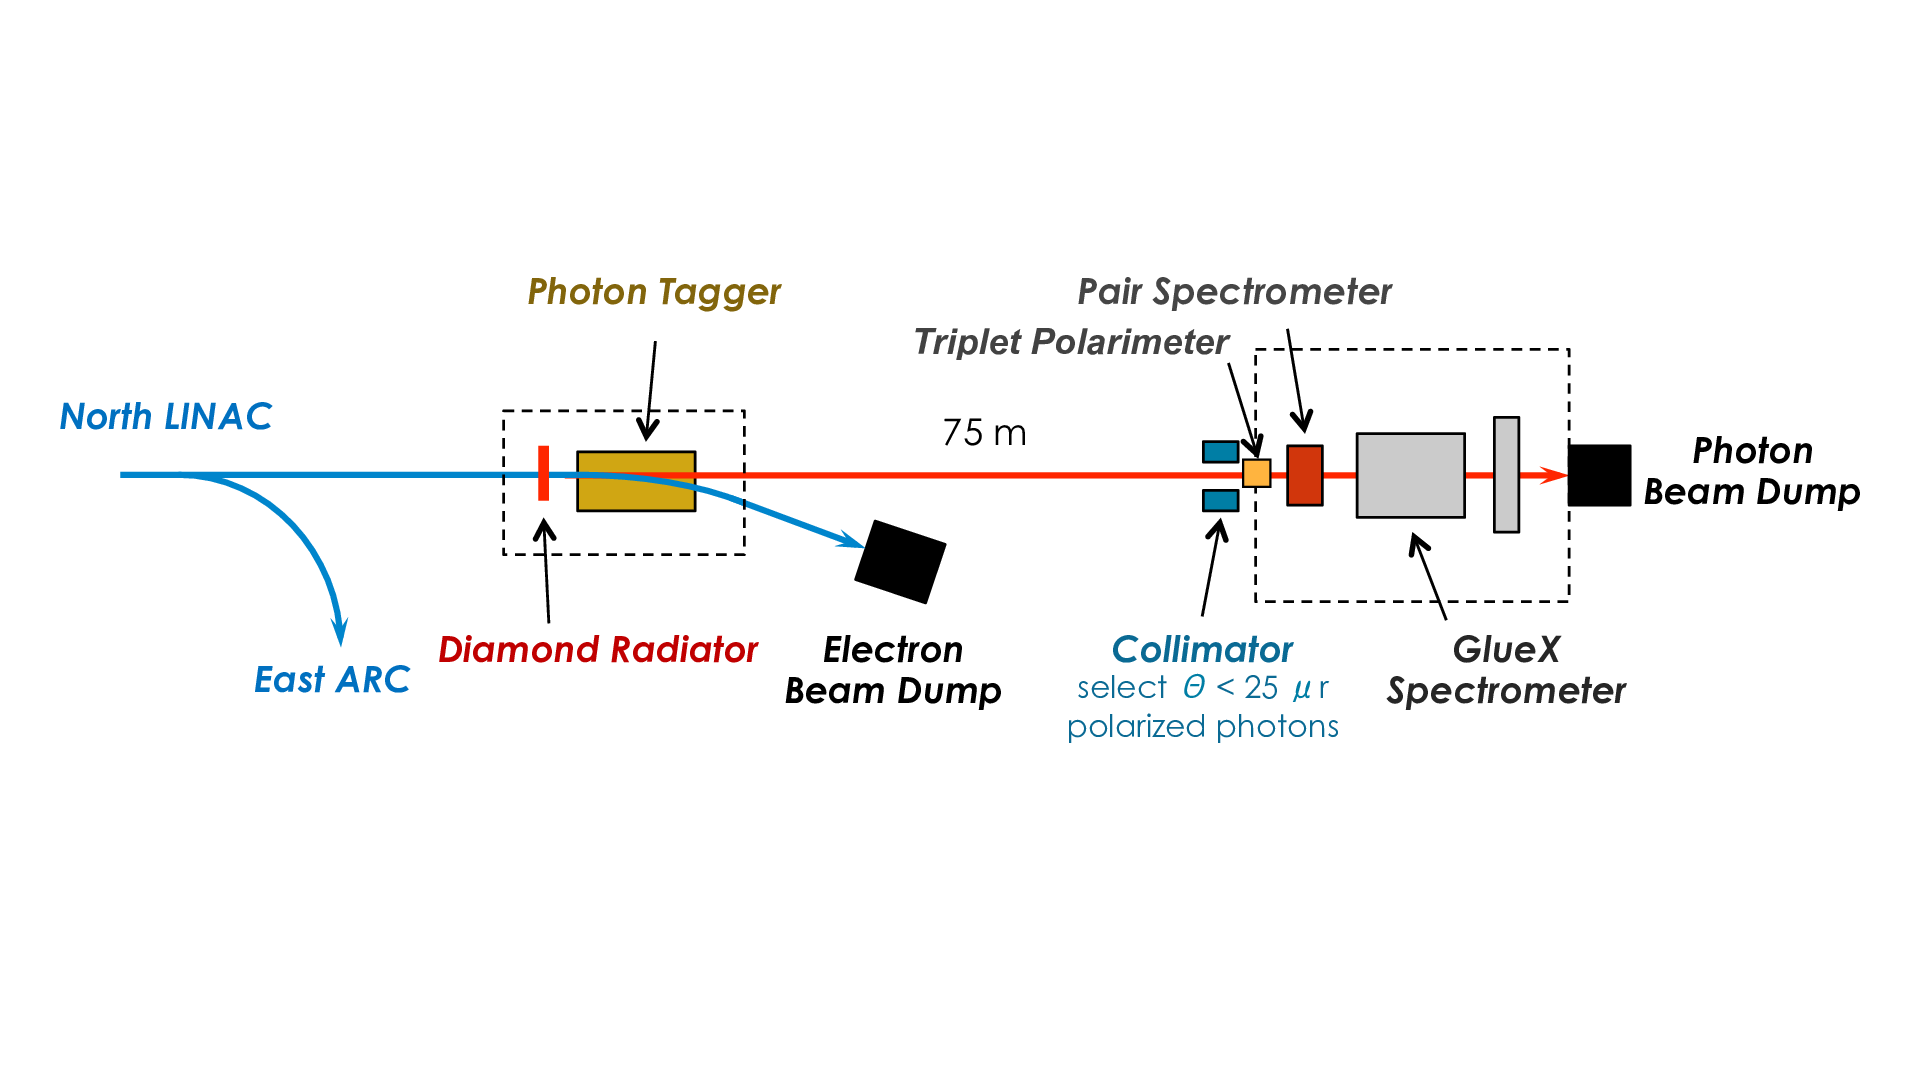
\includegraphics[width=0.95\textwidth]{figures/gluex_beamline.png}
  \end{center}
  \caption{A diagram of the beamline layout of the Triplet Polarimeter (TPOL) and Pair Spectrometer (PS) used to measure the polarization and beam flux.}\label{fig:gluex-beamline}
\end{figure}


To measure the polarization properties of the photon beam as well as the photon flux, the photon beam passes through a thin beryllium foil which induces $e^+e^-$ pair production on some known fraction of the photons (see \Cref{fig:gluex-beamline}). The angular distribution of the produced electrons along with an electron knocked out of the foil medium as part of the pair production process is measured by the Triplet Polarimeter (TPOL) to determine the photon polarization fraction. The Pair Spectrometer (PS) then counts the pair-produced electrons in coincidence with the TAGM and TAGH detectors. A known fraction\footnote{We know the radiation length of the beryllium foil, and this along with the radiator thickness determines the fraction of photons which will pass through without interacting.} of the beam is converted to $e^+e^-$ pairs in this way, allowing for an accurate measurement of the photon flux and the energy dependence of the polarization fraction.

Photons which do not pair-produce in the beryllium radiator interact with a liquid hydrogen cryotarget, which maintains a temperature of $\SI{20.1}{\K}$, allowing the contents to act as a stationary proton target. A set of thin scintillators called the Start Counter (ST) surrounds the target, which captures the initial signals (and azimuthal angles) from reaction products and associates them with the electron radio frequency (RF) beam bunch from which the reaction originated\footnote{The electron beam bunches from the CEBAF arrive every $\SI{4}{\nano\s}$, a rate of $\SI{250}{\mega\hertz}$.}. Any products of the reaction next pass through either the Central Drift Chamber (CDC) or Forward Drift Chamber (FDC) depending on their trajectory (particles within $1^{\circ}$\textendash$10^{\circ}$ of the beamline pass through the FDC, and the detector has partial coverage up to $20^{\circ}$). The CDC is filled with long metal tubes at various orientations, while the FDC chambers are flat disks. Each tube/disk is filled with a gaseous mixture of argon and carbon dioxide\footnote{These particular gases and the mixture ratio are chosen to reduce interfering effects from the magnetic field of the main solenoid.} with a thin wire running through their center of each tube and an array of wires crossing the plane of each disk. The wire and tube/disk faces are held at a voltage differential, and charged particles passing through the chambers ionize the gases inside. The faster-moving electrons move towards the positively charged wires, while the slower-moving ions move towards the tubes/disks. The combination of these signals allows for the reconstruction of the trajectories of each charged particle which passes through each chamber. Both detectors are situated inside a solenoid with a magnetic field around $\SI{2}{\tesla}$, and this field bends the trajectories of charged particles, allowing for proper identification of the sign of the charge as well as the particle's momentum.

The Barrel Calorimeter (BCAL) surrounding the CDC and the Forward Calorimeter (FCAL) in front of the FDC measure the energy of electromagnetic deposits from interactions with charged and neutral particles. This includes photons originating from the decays of light neutral mesons like the $\pi^0$ and $\eta$. Because such neutral particles pass through the CDC and FDC without detection, these calorimeters are necessary for their reconstruction. However, since there are no intermediate trajectories, GlueX is unable to reconstruct the decay vertices of these neutral particles. Since we are studying a reaction with a fully charged final state, this might not seem important. However, in \Cref{sub:neutral-kaon-decay-channels}, we will discuss the study of neutral decays of $K_S^0\to 2\pi^0 \to 4\gamma$, where the reconstruction will be severely limited due to the inability to reconstruct the decay vertex of the $K_S^0$.

There is a final scintillator array called the Time-of-Flight (TOF) detector situated immediately between the FDC and the FCAL. In combination with the ST and the RF timing information from the accelerator, this aids in charged-particle identification via a measurement of the flight time between the two detectors. Additionally, in 2019, an additional detector, the DIRC\footnote{An acronym for Detection of Internally Reflected Cherenkov light} detector was installed between the TOF and FDC to further aid in identification of charged pions and kaons. This detector measures the angle of the cone of Cherenkov radiation emitted by relativistic charged particles, which can be used to ascertain their velocity via the relation $\cos\theta_c \sim 1/v$. When compared to measurements of the particle's momentum, this detector can be used to distinguish pions, kaons, and protons. Further information about the GlueX detector and the DIRC can be found in references \cite{adhikari_gluex_2021} and \cite{ali_installation_2020} respectively.

The data analyzed in this thesis were collected in four separate ``run periods'' across two experiment ``phases'', denoted Phase-I and Phase-II. Phase-I consists of three run periods, notated Spring 2017, Spring 2018, and Fall 2018 by the season and year when data collection began, and Phase-II contains one run period, Spring 2020\footnote{This run technically began at the end of 2019} and is the only dataset which was collected after the DIRC installation. The total luminosity, coherent peak range, and luminosity in the coherent peak for each run period is listed in \Cref{tab:run-info}.


\begin{table}
  \begin{center}
    \begin{tabular}{ccccc}\toprule
      Experiment & Run Period & Luminosity ($E_\gamma > \SI{6.0}{\giga\eV}$) & Coherent Peak Range & Luminosity in Coherent Peak \\\midrule
      Phase-I & Spring 2017 & $\SI{74.7}{\pico\barn^{-1}}$ & $8.2$--$\SI{8.8}{\giga\eV}$ & $\SI{21.8}{\pico\barn^{-1}}$ \\
              & Spring 2018 & $\SI{223.8}{\pico\barn^{-1}}$ & $8.2$--$\SI{8.8}{\giga\eV}$ & $\SI{63.0}{\pico\barn^{-1}}$ \\
              & Fall 2018 & $\SI{141.1}{\pico\barn^{-1}}$ & $8.2$--$\SI{8.8}{\giga\eV}$ & $\SI{40.1}{\pico\barn^{-1}}$ \\\midrule
      Phase-II & Spring 2020 & $\SI{386.2}{\pico\barn^{-1}}$ & $8.0$--$\SI{8.6}{\giga\eV}$ & $\SI{132.4}{\pico\barn^{-1}}$ \\\midrule
      Total & & $\SI{825.8}{\pico\barn^{-1}}$ & & $\SI{257.3}{\pico\barn^{-1}}$ \\\bottomrule
    \end{tabular}
    \caption{Summary of total luminosity and total luminosity in the coherent peak for each run period.}\label{tab:run-info}
  \end{center}
\end{table}

The entire GlueX detector has been simulated with Geant4. Due to small changes and updates to the detector and its simulation between run periods, we will treat these datasets separately during the analysis, only presenting combined results in summary. Therefore, when generating Monte Carlo simulated data to model detector acceptance, each run period must be simulated separately.

\subsection{Particle Identification and the GlueX Kinematic Fit}\label{sub:particle-identification-and-the-gluex-kinematic-fit}
Unsurprisingly, data collected from the GlueX detector mostly contains reaction topologies (the set of initial\-/, intermediate\-/, and final\-/state particles) which are not the channel of interest in this thesis. Additionally, due to the unavoidable finite resolution of each detector, the measured quantities such as the momentum of each particle might not exactly align with physical expectations (such as four-momentum conservation). For these reasons, we need to filter the detected data to just events which match our desired topology and kinematically fit the observables such as particle masses, decay vertices, and four-momenta with constraints that enforce conservation laws and other desirable properties.

This process begins with particle reconstruction, where the raw detector data is transformed into charged particle tracks (from the drift chambers), photon showers (from the calorimeters), and some timing data from the ST and TOF. Next, the charged tracks are matched up with their respective showers from the calorimeters, and the remaining showers are labeled as ``neutral showers'' originating from photons (or possibly large neutral particles like neutrons). At this stage, no particle identification is assigned to the charged and neutral tracks.

\subsubsection{Particle Identification Cuts}

The next stage involves filtering through reconstructed tracks to find events which match our topology. First, we apply some basic selections to the track data, including a requirement that neutral showers must have an energy of at least $\SI{100}{\mega\eV}$ and neutral showers in the BCAL must be detected in at least two detector cells. Timing cuts are then applied to whichever detector gives the best timing information (the order being BCAL, TOF, FCAL, ST). By timing, we mean the difference between the time measured in the detector and the time of the RF beam bunch measured in the TAGH/TAGM. Each set of charged tracks is identified with each charged particle in the topology (events with too many or too few charged tracks are excluded). Each hypothetical identification is then subjected to cuts on the energy lost in the drift chambers or deposited in the calorimeters. Since there are no ``missing'' final-state particles (such as a neutron) in our reaction, an additional cut is made on the missing energy (the difference between the initial energy from the beam photon and the summed energy of the final-state particles). Finally, cuts are made on the invariant mass of some particles, as well as the missing mass (squared) for the step of the reaction from which the particle originated. For example, in the reaction $\gamma p \to K_S^0 K_S^0 p \to \pi^+\pi^-\pi^+\pi^- p$, a missing mass cut applied to the recoil proton would use the difference between the (squared) invariant mass of $\gamma p$ and $4\pi p$, but the missing mass cuts applied to one of th $\pi^+$ would involve the difference between the (squared) invariant mass of the $K_S^0$ it originated from and the decay product $\pi^+\pi^-$. A summary of these particle identification (PID) cuts can be seen in \Cref{tab:pid-cuts}.

\begin{table}
  \begin{center}
    \begin{tabular}{cccc}\toprule
      Particle & Selected Values & Unit & Detector \\\midrule
      \gamma & $-1.5 \leq \Delta t_{\text{RF}} \leq 1.5$ & $\si{\nano\s}$ & BCAL\\
             & $-2.5 \leq \Delta t_{\text{RF}} \leq 2.5$ & $\si{\nano\s}$ & FCAL\\
             & $-0.1 \leq \text{MM}^2 \leq 0.1$ & $\si{(\giga\eV/c^2)^2}$ & N/A\\\midrule
      \pi^{\pm} & $-1.0 \leq \Delta t_{\text{RF}} \leq 1.0$ & $\si{\nano\s}$ & BCAL\\
                & $-0.5 \leq \Delta t_{\text{RF}} \leq 0.5$ & $\si{\nano\s}$ & TOF\\
                & $-2.0 \leq \Delta t_{\text{RF}} \leq 2.0$ & $\si{\nano\s}$ & FCAL\\
                & $-2.5 \leq \Delta t_{\text{RF}} \leq 2.5$ & $\si{\nano\s}$ & ST\\
                & $\dv{E}{x} < \exp[-7.0\abs{\vec{p}} + 3.0] + 6.2$ & $\si{\kilo\eV/\centi\m}$ ($\dv{E}{x}$), $\si{\giga\eV/c}$ ($\abs{\vec{p}}$) & CDC \\
                & $-1.0 \leq \text{MM}^2 \leq 1.0$ & $\si{(\giga\eV/c^2)^2}$ & N/A\\\midrule
      p & $-1.0 \leq \Delta t_{\text{RF}} \leq 1.0$ & $\si{\nano\s}$ & BCAL\\
                & $-0.6 \leq \Delta t_{\text{RF}} \leq 0.6$ & $\si{\nano\s}$ & TOF\\
                & $-2.0 \leq \Delta t_{\text{RF}} \leq 2.0$ & $\si{\nano\s}$ & FCAL\\
                & $-2.5 \leq \Delta t_{\text{RF}} \leq 2.5$ & $\si{\nano\s}$ & ST\\
                & $\dv{E}{x} > \exp[-4.0\abs{\vec{p}} + 2.25] + 1.0$ & $\si{\kilo\eV/\centi\m}$ ($\dv{E}{x}$), $\si{\giga\eV/c}$ ($\abs{\vec{p}}$) & CDC \\
                & $-0.5 \leq \text{MM}^2 \leq 4.41$ & $\si{(\giga\eV/c^2)^2}$ & N/A\\\midrule
      $\pi^0$ & $0.08 \leq \text{IM} \leq 0.19$ & $\si{\giga\eV/c^2}$ & N/A\\
              & $-1.0 \leq \text{MM}^2 \leq 1.0$ & $\si{(\giga\eV/c^2)^2}$ & N/A\\\midrule
      $K_S^0$ & $0.3 \leq \text{IM} \leq 0.7$ & $\si{\giga\eV/c^2}$ & N/A\\
              & $-1.0 \leq \text{MM}^2 \leq 2.0$ & $\si{(\giga\eV/c^2)^2}$ & N/A\\\midrule
      N/A & $-3.0 \leq \text{ME} \leq 3.0$ & $\si{\giga\eV}$ & N/A\\\bottomrule
    \end{tabular}
    \caption{PID cuts used in event reconstruction. $\text{MM}^2$ corresponds to the missing mass squared, $\text{IM}$ corresponds to the invariant mass, and $ME$ corresponds to the total missing energy.}\label{tab:pid-cuts}
  \end{center}
\end{table}

\subsubsection{Kinematic Fit}

The final stage of reconstruction invokes a kinematic fit (KinFit) over data which has passed all PID cuts. This kinematic fit minimizes the following objective function:

\begin{equation}
  \chi^2(\vec{\eta},\vec{\xi}) = (\vec{y} - \vec{\eta})^\intercal \mathbf{V}_{\vec{y}}^{-1}(\vec{y} - \vec{\eta}) + 2 \vec{\lambda}^\intercal\vec{f}(\vec{\eta},\vec{\xi})
  \label{eq:kinfit-chi}
\end{equation}
where $\vec{y}$ are the experimentally measured values of observables $\vec{\eta}$, $\mathbf{V}_{\vec{y}}$ is the covariance matrix of the measured $\vec{y}$, $\vec{f}(\vec{\eta},\vec{\xi}) = 0$ are constraints applied to the system with additional free parameters $\vec{\xi}$ (which do not correspond to measured observables), and $\lambda$ are unknown Lagrange multipliers for said constraints. Since we wish to minimize $\chi^2$, we first take derivatives with respect to each set of free parameters,

\begin{align}
  \pdv{\chi^2}{\vec{\eta}} &= \mathbf{V}_{\vec{y}}^{-1}(\vec{\eta}-\vec{y}) + \left(\pdv{\vec{f}}{\vec{\eta}}\right)^\intercal\vec{\lambda} \label{eq:kinfit-dxdeta}\\
  \pdv{\chi^2}{\vec{\lambda}} &= \vec{f}(\vec{\eta},\vec{\xi}) \label{eq:kinfit-dxdlambda}\\
  \pdv{\chi^2}{\vec{\xi}} &= \left(\pdv{\vec{f}}{\vec{\xi}}\right)^\intercal\vec{\lambda} \label{eq:kinfit-dxdxi}
\end{align}

To find an extrema, we set these each to $\vec{0}$ and solve. At GlueX, the KinFit uses the Newton-Raphson method. First, we Taylor expand the constraint equations to first order,

\begin{equation}
  \vec{f}(\vec{\eta},\vec{\xi}) \approx \vec{f}(\vec{\eta}_0,\vec{\xi}_0) + \left(\pdv{\vec{f}}{\vec{\eta}}\right)\eval_{\vec{\eta}_0,\vec{\xi}_0}\left(\vec{\eta} - \vec{\eta}_0\right) + \left(\pdv{\vec{f}}{\vec{\xi}}\right)\eval_{\vec{\eta}_0,\vec{\xi}_0}\left(\vec{\xi} - \vec{\xi}_0\right)
\end{equation}

Assuming $\vec{\eta}_0$ and $\vec{\xi}_0$ are near the true minimum, we can set up an iterative method of approach,

\begin{equation}
  \vec{f}_i + \left(\pdv{\vec{f}}{\vec{\eta}}\right)_i\left(\vec{\eta}_{i+1} - \vec{\eta}_i\right) + \left(\pdv{\vec{f}}{\vec{\xi}}\right)_i\left(\vec{\xi}_{i+1} - \vec{\xi}_i\right) = \vec{0}
\end{equation}

To carry out an iteration, we need to determine the next step in each of the free directions $\vec{\eta}_{i+1}$ and $\vec{\xi}_{i+1}$. We start by writing the iterative forms of \Cref{eq:kinfit-dxdeta,eq:kinfit-dxdxi} as

\begin{align}
  \mathbf{V}_{\vec{y}}^{-1}(\vec{\eta}_{i+1} - \vec{y}) + \left(\pdv{\vec{f}}{\vec{\eta}}\right)^\intercal_i \vec{\lambda}_{i+1} &= 0 \label{kinfit-dxdeta-iter} \\
  \left(\pdv{\vec{f}}{\vec{\xi}}\right)^\intercal_i \vec{\lambda}_{i+1} &= 0 \label{kinfit-dxdxi-iter}
\end{align}

We can rearrange \Cref{kinfit-dxdeta-iter} as

\section{Data Selection for the $K_SK_S$ Channel}\label{sec:data-selection}
These reconstruction steps all take place before we interact with the data. The cut values in \Cref{tab:pid-cuts} are loose, and there is surely background remaining. To remove it, we first must know the potential sources of backgrounds in the $K_S^0K_S^0$ channel, which we will do by simulating a large set of events with many different reaction topologies, passing them through reconstruction, and then comparing the distributions of each topology which makes it through. The simulation uses the \texttt{bggen} Monte Carlo generator, which in turn uses \texttt{PYTHIA}~\cite{Bierlich2022} for event generation and a GlueX implementation of \texttt{Geant4}~\cite{Allison2006,Allison2016,Agostinelli2003}. The relative proportions of reaction topologies do not necessarily reflect the production cross sections we expect to see in data (for instance, there are no resonances included in the $K_S^0K_S^0$ channel), but they should give us a good idea of the kinds of topologies which leak into this channel.

\begin{figure}
  \begin{center}
    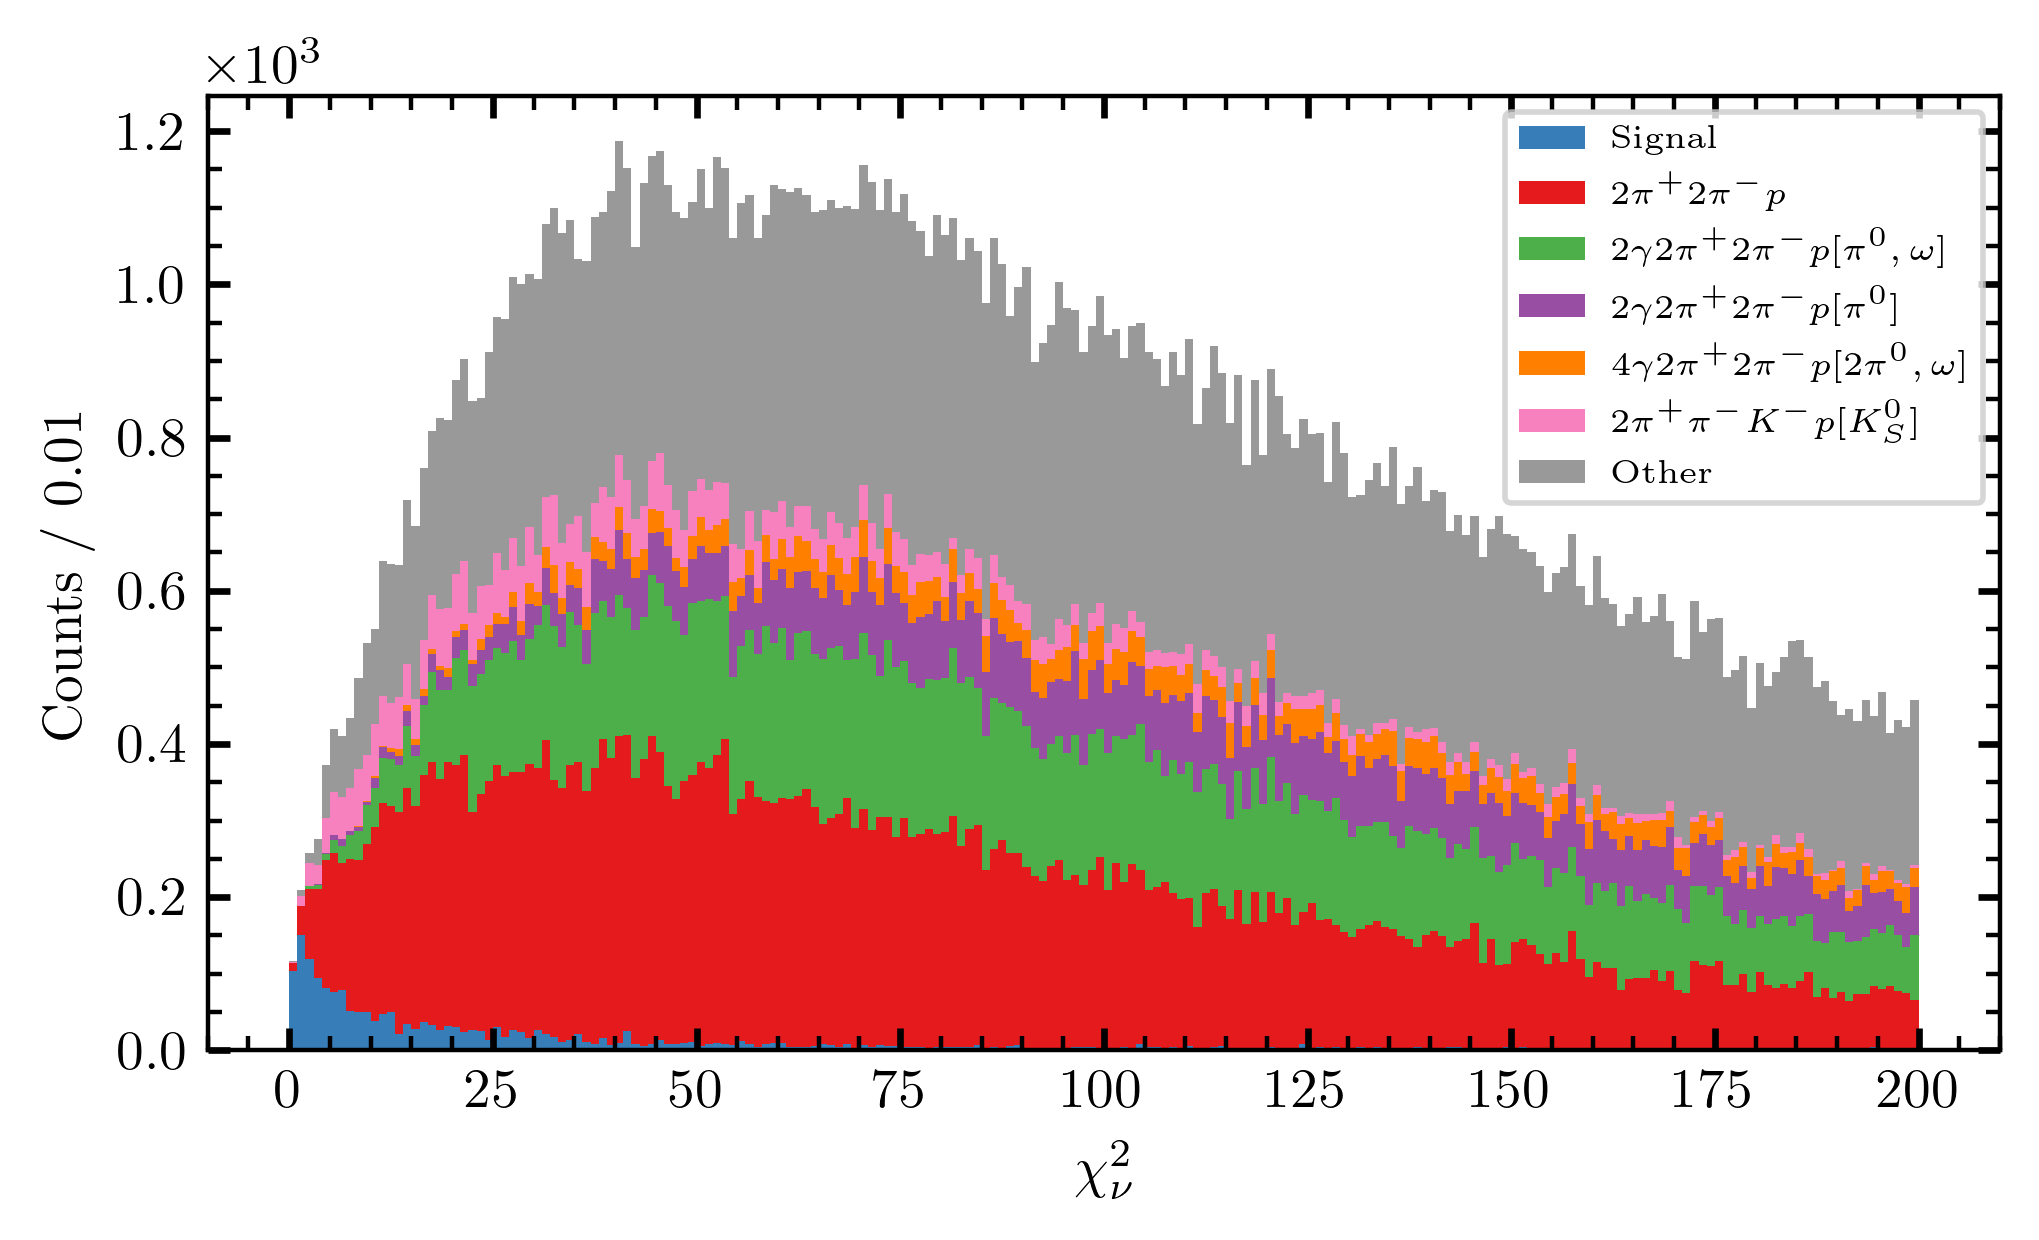
\includegraphics[width=0.8\textwidth]{figures/bggen_chisqdof.png}
  \end{center}
  \caption{The reduced $\chi^2$ statistic of the GlueX kinematic fit for the \texttt{bggen} simulation. The stacked histogram contains the signal channel, $K_S^0K_S^0$ as well as the five most prominent background components.}\label{fig:bggen-chisqdof}
\end{figure}

We will first look at the performance of the GlueX kinematic fit on \texttt{bggen} data in \Cref{fig:bggen-chisqdof}. In this plot, we see the signal, which predictably peaks at $\chi^2_\nu \sim 1$, as well as several background topologies. These topologies are labeled by their final state along with any intermediate decaying resonances in square brackets. The top five potential backgrounds, in order of the size of their contribution after reconstruction, are as follows. First, $2\pi^+2\pi^- p$ shares the final state of the signal channel but does not contain any $K_S^0$ intermediate decays. Second, $2\gamma 2\pi^+ 2\pi^- p [\pi^0, \omega]$ contains an $\omega$ which decays to $\pi^+\pi^-\pi^0$, followed by the $\pi^0$ decaying to $2\gamma$. The addition of extra photons is common in these backgrounds, since missing the photon detections makes the final state identical to the signal. The next two reactions, $2\gamma 2\pi^+ 2\pi^- p [\pi^0]$ and $4\gamma 2\pi^+ 2\pi^- p [2\pi^0, \omega]$ both include an undetected $\pi^0$. Finally, $2\pi^+\pi^- K^- p[K_S^0]$ contains a $K^-$ which is mistakenly identified as a $\pi^-$.

It seems sensible to make a cut on the $\chi^2_\nu$ of the kinematic fit, since the signal is clearly favored at lower values. Below $\chi^2_\nu < 10$, the background topologies are dominated by the $4\pi$ channel which does not contain kaons. As such, this source of background will be our primary focus for removal.

\subsection{Fiducial Cuts}\label{sub:fiducial-cuts}
To get a clearer picture of the data, we will first make a loose cut selecting only events with $\chi^2_\nu < 10$. We can then generate phase-space Monte Carlo for the $4\pi$ background reaction and search for potential ways to separate it from the signal by comparing the distributions of common kinematic variables.

\begin{figure}
  \begin{center}
    \includegraphics[width=0.8\textwidth]{ext/analysis/plots/chisqdof_combined_None_None_None.png}
  \end{center}
  \caption{The normalized distributions of $\chi^2_\nu$ for the true data and phase-space signal and $4\pi$ background Monte Carlo.}\label{fig:data-combined-chisqdof}
\end{figure}

In \Cref{fig:data-combined-chisqdof}, we can see the various distributions of the data and each simulated channel. Unfortunately, the data distribution resembles the $4\pi$ background distribution much better than the signal Monte Carlo, but now we also know that the signal decays rapidly at higher values of $\chi^2_\nu$, so a tighter selection might improve the signal-to-background ratio, even if we cannot immediately see a peak in the data near unity. It is difficult to choose a value at which to cut in this variable, but the choice is largely arbitrary. We will be using a statistical weighting method in \Cref{sec:splot} to subtract the non-strange background represented by the $4\pi$ Monte Carlo, but we must make some choice on $\chi^2_\nu$ before that step in the analysis to reduce other backgrounds mentioned in \Cref{sec:data-selection}. For simplicity, we will conduct the entire analysis using a selection of $\chi^2_\nu < 3.0$, and we will later select several other values on either side of this cut to study its systematic effect in \Cref{sec:systematic-studies}.

As mentioned in \Cref{sec:data-selection}, the asymmetry in missing energy in \Cref{fig:me-combined} likely comes from background channels with photons which were missed in reconstruction. The selection on $\chi^2_\nu$ greatly reduces the contributions from these backgrounds, as can be seen in \Cref{fig:me-combined-chisqdof-3.0}

\begin{figure}
  \begin{center}
    \includegraphics[width=0.8\textwidth]{ext/analysis/plots/me_combined_chisqdof_3.0_None_None_None.png}
  \end{center}
  \caption{Normalized distributions of the missing energy ($E_i - E_f$) for data, phase-space signal Monte Carlo, and $4\pi$ background Monte Carlo after a selection of $\chi^2_\nu < 3.0$ is applied.}\label{fig:me-combined-chisqdof-3.0}
\end{figure}


\begin{figure}
  \begin{center}
    \includegraphics[width=0.8\textwidth]{ext/analysis/plots/mm2_combined_chisqdof_3.0_None_None_None.png}
  \end{center}
  \caption{The normalized distributions of missing mass squared for the true data and phase-space signal and $4\pi$ background Monte Carlo after a selection of $\chi^2_\nu < 3.0$ is applied.}\label{fig:mm2-combined-chisqdof-3.0}
\end{figure}

Another common selection which can be made is on the squared missing mass of an event, which is just the square of the difference between the initial- and final-state four-momenta. This variable, visualized in \Cref{fig:mm2-combined-chisqdof-3.0}, predictably peaks at zero for the data, signal Monte Carlo, and background Monte Carlo, and the overall distributions for the signal and backgound simulated events are nearly identical. This indicates that a selection on this variable would not be very useful at distinguishing the signal from the background.

There are two more minor selections which we will perform on the data. The first is a selection on the invariant mass of $K_S^0K_S^0$ at $\text{IM} < \SI{2.0}{\giga\electronvolt}$. This is done because models we use later to describe the data do not include any higher-mass resonances, and data past this point causes issues with the mass-dependent fits in \Cref{sec:mass-dependent-fits}. The other is a selection on the $z$-vertex of the target proton. We know the exact location of the target with respect to the detector, and we only want to deal with events which we know originated inside this target. The distribution of the $z$-vertex values can be seen in \Cref{fig:protonz-combined}. We will select events with $\SI{50}{\centi\meter} < z < \SI{80}{\centi\meter}$, as this is the known length and position of the target relative to the detector elements. While there is an indication of events in the signal Monte Carlo in the regions which are removed, we know that while these events originated from the target, their $z$-vertex has been misidentified, so we should remove them anyway.


\begin{figure}
  \begin{center}
    \includegraphics[width=0.8\textwidth]{ext/analysis/plots/protonz_combined_None_None_None.png}
  \end{center}
  \caption{The normalized distributions of the target proton $z$-vertex for the true data and phase-space signal and $4\pi$ background Monte Carlo (no cuts applied).}\label{fig:protonz-combined}
\end{figure}

An impetus for studying this channel was originally a search for excited hyperons\textemdash baryons with strange quark content. In particular, $\Sigma^+$ resonances should form in the invariant mass distribution of $K_S^0 p$, where the other kaon is required to conserve strangeness in the strong production of this baryon. There is a symmetry between the identical kaons which must first be accounted for. We could pair either kaon with the proton to form the $\Sigma^+$, but there is a more likely pairing which can be found by first recognizing that the heavier hyperon will generally move more backwards in the center-of-momentum frame than the lighter bachelor $K_S^0$. Therefore, the kaon which is moving in a further backward direction is more likely to correspond with the hyperon decay candidate. We can sort the kaons by their $\cos\theta$ in the center-of-momentum frame and call the more backward-going kaon $K_{S,B}^0$. The invariant mass spectrum of $K_{S,B}^0 p$ can be seen in \Cref{fig:baryon-mass-data-pz-chisqdof-3.0}. The enhancement around $\SI{1.7}{\giga\electronvolt}$ likely corresponds to some combination of the $\Sigma^+(1660)$, $\Sigma^+(1670)$, $\Sigma^+(1750)$, and $\Sigma^+(1775)$ resonances. We do not see much indication of states above $\SI{2}{\giga\electronvolt}$.

\begin{figure}
  \begin{center}
    \includegraphics[width=0.8\textwidth]{ext/analysis/plots/baryon_mass_data_pz_chisqdof_3.0_None_None_None.png}
  \end{center}
  \caption{The mass distribution of the backward-going $K_S^0$ combined with the proton. Only the proton $z$-vertex and $\chi^2_\nu$ cuts are applied, as the cut on invariant mass reduces much of the visible baryon contribution which tends to show up at higher $K_S^0K_S^0$ invariant mass.}\label{fig:baryon-mass-data-pz-chisqdof-3.0}
\end{figure}


This angle also gives us a handle on separating baryonic and mesonic topologies. If we plot the $\cos\theta$ of $K_{S,B}^0$ against the invariant mass of $K_{S,B}^0 p$, as in \Cref{fig:ksb-costheta-v-baryon-mass-data-pz-chisqdof-3.0}, we find a strong and somewhat expected dependence. The majority of the baryonic contribution occurs at angles with $\cos\theta < 0$. Likewise, the mesonic contribution is mostly confined to angles of $\cos\theta > 0$, as seen in figures \Cref{fig:ksb-costheta-v-meson-mass-data-pz-chisqdof-3.0,fig:meson-mass-data-pz-masscut-chisqdof-3.0-mesons}. While it may not be obvious that there even are meson resonances here, we will see their contributions much more clearly after the statistical weighting procedures defined in \Cref{sec:splot} have been applied, after which we will revisit these plots. We will also conduct our analysis without this selection in \Cref{sec:systematic-studies} for completeness. We can also isolate the baryon contributions by reversing this selection, and the result of this is seen in \Cref{fig:baryon-mass-data-pz-masscut-chisqdof-3.0-baryons}.

\begin{figure}
  \begin{center}
    \includegraphics[width=0.8\textwidth]{ext/analysis/plots/ksb_costheta_v_baryon_mass_data_pz_chisqdof_3.0_None_None_None.png}
  \end{center}
  \caption{The center-of-momentum azimuthal angle of $K_{S,B}^0$ plotted against the invariant mass of $K_{S,B}^0 p$. The baryonic contribution occurs mostly at far backward angles, while mesons appear at the far forward angles. Only the proton $z$-vertex and $\chi^2_\nu$ cuts are applied, as the cut on invariant mass reduces much of the visible baryon contribution which tends to show up at higher $K_S^0K_S^0$ invariant mass.}\label{fig:ksb-costheta-v-baryon-mass-data-pz-chisqdof-3.0}
\end{figure}

\begin{figure}
  \begin{center}
    \includegraphics[width=0.8\textwidth]{ext/analysis/plots/ksb_costheta_v_meson_mass_data_pz_chisqdof_3.0_None_None_None.png}
  \end{center}
  \caption{The center-of-momentum azimuthal angle of $K_{S,B}^0$ plotted against the invariant mass of $K_S^0K_S^0$. The baryonic contribution occurs mostly at far backward angles, while mesons appear at the far forward angles. Only the proton $z$-vertex and $\chi^2_\nu$ cuts are applied, as the cut on invariant mass reduces much of the visible baryon contribution which tends to show up at higher $K_S^0K_S^0$ invariant mass.}\label{fig:ksb-costheta-v-meson-mass-data-pz-chisqdof-3.0}
\end{figure}

\begin{figure}
  \begin{center}
    \includegraphics[width=0.8\textwidth]{ext/analysis/plots/meson_mass_data_pz_masscut_chisqdof_3.0_mesons_None_None.png}
  \end{center}
  \caption{The invariant mass of $K_S^0K_S^0$ across all datasets after all fiducial selections are applied.}\label{fig:meson-mass-data-pz-masscut-chisqdof-3.0-mesons}
\end{figure}

\begin{figure}
  \begin{center}
    \includegraphics[width=0.8\textwidth]{ext/analysis/plots/baryon_mass_data_pz_masscut_chisqdof_3.0_baryons_None_None.png}
  \end{center}
  \caption{The invariant mass of $K_S^0K_S^0$ across all datasets after all fiducial selections are applied, but with the baryon rejection cut reversed to select baryons.}\label{fig:baryon-mass-data-pz-masscut-chisqdof-3.0-baryons}
\end{figure}

Finally, we can examine some of the typical detector plots which are used to separate and identify charged particles, namely the energy loss from these charged tracks as measured by the FDC and CDC. As we can see in \Cref{fig:dedx-v-p-cdc-proton-pz-masscut-chisqdof-3.0-mesons,fig:dedx-v-p-cdc-pions-pz-masscut-chisqdof-3.0-mesons}, the data recorded in the CDC after the previous fiducial selections is in agreement with that of the signal Monte Carlo. Next, in the FDC, we do not retain a significant number of proton tracks due to the baryon rejection cut, but enough pions are recorded in the FDC to reveal a discrepancy between data and Monte Carlo, as seen in \Cref{fig:dedx-v-p-fdc-pions-pz-masscut-chisqdof-3.0-mesons}. The signal Monte Carlo here tells us that out of the two horizontal bands, the upper band coincides with real pions, while the other band is likely some background. While the total number of pions which end up in the FDC is small, it is still important to remove these background events, and we will do so with a selection on the energy loss {\color{red}Note to committee, this is a work-in-progress which we do not expect will significantly effect the rest of the thesis}.


\begin{figure}
    \centering
    \begin{subfigure}{0.45\textwidth}
        \includegraphics[width=\linewidth]{ext/analysis/plots/dedx_v_p_cdc_proton_sigmc_pz_masscut_chisqdof_3.0_mesons_None_None.png}
        \caption{Signal Monte Carlo}
    \end{subfigure}
    \hfill
    \begin{subfigure}{0.45\textwidth}
        \includegraphics[width=\linewidth]{ext/analysis/plots/dedx_v_p_cdc_proton_data_pz_masscut_chisqdof_3.0_mesons_None_None.png}
        \caption{Data}
    \end{subfigure}
    \caption{The energy loss in the CDC for protons after all fiducial cuts are applied.}\label{fig:dedx-v-p-cdc-proton-pz-masscut-chisqdof-3.0-mesons}
\end{figure}

\begin{figure}
    \centering
    \begin{subfigure}{0.45\textwidth}
        \includegraphics[width=\linewidth]{ext/analysis/plots/dedx_v_p_cdc_piplus1_sigmc_pz_masscut_chisqdof_3.0_mesons_None_None.png}
        \caption{Signal Monte Carlo}
    \end{subfigure}
    \hfill
    \begin{subfigure}{0.45\textwidth}
        \includegraphics[width=\linewidth]{ext/analysis/plots/dedx_v_p_cdc_piplus1_data_pz_masscut_chisqdof_3.0_mesons_None_None.png}
        \caption{Data}
    \end{subfigure}
    \vspace{1em}
    \begin{subfigure}{0.45\textwidth}
        \includegraphics[width=\linewidth]{ext/analysis/plots/dedx_v_p_cdc_piminus1_sigmc_pz_masscut_chisqdof_3.0_mesons_None_None.png}
        \caption{Signal Monte Carlo}
    \end{subfigure}
    \hfill
    \begin{subfigure}{0.45\textwidth}
        \includegraphics[width=\linewidth]{ext/analysis/plots/dedx_v_p_cdc_piminus1_data_pz_masscut_chisqdof_3.0_mesons_None_None.png}
        \caption{Data}
    \end{subfigure}
    \caption{The energy loss in the CDC for pions after all fiducial cuts are applied.}\label{fig:dedx-v-p-cdc-pions-pz-masscut-chisqdof-3.0-mesons}
\end{figure}

\begin{figure}
    \centering
    \begin{subfigure}{0.45\textwidth}
        \includegraphics[width=\linewidth]{ext/analysis/plots/dedx_v_p_fdc_piplus1_sigmc_pz_masscut_chisqdof_3.0_mesons_None_None.png}
        \caption{Signal Monte Carlo}
    \end{subfigure}
    \hfill
    \begin{subfigure}{0.45\textwidth}
        \includegraphics[width=\linewidth]{ext/analysis/plots/dedx_v_p_fdc_piplus1_data_pz_masscut_chisqdof_3.0_mesons_None_None.png}
        \caption{Data}
    \end{subfigure}
    \vspace{1em}
    \begin{subfigure}{0.45\textwidth}
        \includegraphics[width=\linewidth]{ext/analysis/plots/dedx_v_p_fdc_piminus1_sigmc_pz_masscut_chisqdof_3.0_mesons_None_None.png}
        \caption{Signal Monte Carlo}
    \end{subfigure}
    \hfill
    \begin{subfigure}{0.45\textwidth}
        \includegraphics[width=\linewidth]{ext/analysis/plots/dedx_v_p_fdc_piminus1_data_pz_masscut_chisqdof_3.0_mesons_None_None.png}
        \caption{Data}
    \end{subfigure}
    \caption{The energy loss in the FDC for pions after all fiducial cuts are applied. {\color{red}Note to committee: The extra structure here will be addressed with a cut, but it will have minimial impact on this thesis and take several days to reprocess data. Expect an update to this section.}}\label{fig:dedx-v-p-fdc-pions-pz-masscut-chisqdof-3.0-mesons}
\end{figure}

In total, we have the fiducial selections on the data illustrated in \Cref{tab:fiducial-cuts}.

\begin{table}
  \begin{center}
    \begin{tabular}{cc}\toprule
      Variable & Selected Values \\\midrule
      $\chi^2_\nu$ & $\chi^2_\nu < 3.0$ \\
      Mass of $K_S^0K_S^0$ & $ m < \SI{2.0}{\giga\electronvolt} $ \\
      Target proton-$z$ & $\SI{50}{\centi\meter} < z < \SI{80}{\centi\meter}$ \\
      $\cos\theta_{\text{CM}}$ of $K_{S,B}^0$ & $ \cos\theta_{\text{CM}} > 0.0 $ \\\bottomrule
    \end{tabular}
    \caption{Fiducial cuts performed after event reconstruction.}\label{tab:fiducial-cuts}
  \end{center}
\end{table}

\subsection{Accidental Subtraction}\label{sub:accidental-subtraction}
Before we can discuss subtracting the $4\pi$ background, we need to deal with another source of background which we cannot avoid with cuts. As mentioned in \Cref{subsub:combos}, each event in the dataset holds multiple ``combos''\textemdash alternate hypotheses for the set or ordering of the particles which make up the topology. For example, in the $K_S^0K_S^0$ final state, there are two identical $\pi^+$ and $\pi^-$ particles. The choice of which $\pi^+$ goes with which $\pi^-$ to form each kaon is partially constrained by the kinematic fit, but in the case where both pion combinations yield results which pass through the entire reconstruction and particle identification process, both are included as separate combos in the same event. The fiducial selections we performed in \Cref{sub:fiducial-cuts} eliminate many of these combos, since the incorrect combinations will sometimes have very high $\chi^2_\nu$, but there may be some remaining at the end of these selections. For this combinatoric case, we can reduce the effect of incorrect combinations by only selecting the combo with the lowest $\chi^2_\nu$ in each event. While this does not guarantee that we will have the correct combination, it will prevent us from double-counting, and it is more likely that the best $\chi^2_\nu$ is the true event.

Additionally, we can get combos from different beam photon combinations. If multiple tagged photons have energies which are compatible with the reaction, each is included as a separate combo. It can also be the case that the true photon was simply not reconstructed, and some incorrect photon which was close enough was matched with the combo instead. In either case, we have multiple combos which do not correspond to true events. We call both of these cases ``accidental'' combos. To account for this, we first recall that the accelerator produces beam bunches every $\SI{4}{\nano\second}$ in radio-frequency (RF) bunches. A beam bunch consistent with a given reconstructed event is labeled ``in-time'', while the surrounding bunches are called ``out-of-time''. We can reduce the impact of these accidental combos by estimating the contribution they have on the in-time events and using out-of-time events as a negatively-weighted background estimation. Since the in-time accidentals are indistinguishable from true events, we must use other types of events which also pass through kinematic selections in our subtraction, and the out-of-time events can be used for this purpose. The estimation of the scaling for these out-of-time contributions has been calculated via systematic studies of the TAGM/TAGH components. For our data, we choose to include eight bunches of accidentals, although we cut out the bunches neighboring the in-time peak to avoid including in-time events in our subtraction. The distribution of the difference in RF times with respect to the event time is shown in \Cref{fig:rf-unweighted-data-pz-masscut-chisqdof-3.0-mesons}. In this figure, the in-time events are located in the peak centered at zero, and we cut the peaks at $\pm \SI{4}{\nano\second}$ on either side\footnote{The exact value used is $\SI{4.008016032}{\nano\second}$.}. The remaining three out-of-time peaks on either side are given a negative weight (approximately $1/6$th for each) while the in-time peak gets a weight of $1$.

To unify this accidental subtraction with the combinatoric reduction done by selecting the best $\chi^2_\nu$, we first perform the $\chi^2_\nu$ selection, which reduces each event to a single combo (some of which might be in the out-of-time peaks), and then we carry out the accidental subtraction. At this stage, the only background which remains unaccounted for is that of incorrect topologies disguised as our signal.

\begin{figure}
  \begin{center}
    \includegraphics[width=0.8\textwidth]{ext/analysis/plots/rf_unweighted_data_pz_masscut_chisqdof_3.0_mesons_None_None.png}
  \end{center}
  \caption{The time difference between the RF time recorded by the tagger and the event time. The main peak in the middle contains in-time events while the three peaks on either side are the out-of-time events added to the dataset to simulate accidental combos in the main peak.}\label{fig:rf-unweighted-data-pz-masscut-chisqdof-3.0-mesons}
\end{figure}

\section{sPlot Weighting}\label{sec:splot}
At this stage in the analysis, we have no more simple cuts which can improve the signal-to-background ratio in the dataset, but we know there must still be background remaining, as is indicated by the excess events with small kaon rest-frame lifetimes seen in \Cref{fig:rfl-pre-splot}. In this figure, we see that one of the intrinsic properties of a $K_S^0$, its well-known lifetime around $\SI{89.54}{\pico\second}$, is not present in the data. Rather, we seem to have at least two exponential slopes in the rest-frame lifetime distribution of each kaon, one which is close to what we see in signal Monte Carlo, and another which is similar to the $4\pi$ background Monte Carlo. The $K_S^0$ lifetime comes from the fact that it contains a strange quark but decays to two non-strange mesons, and a weak interaction is required for this to occur. While we might not know the exact process which creates the $4\pi$ background, we can assume a strong interaction produces the pions, which should happen several orders of magnitude faster than the $K_S^0$ decay. Due to the resolution of the detector, we still expect these events to appear to have some non-zero distribution in rest-frame lifetime when we mistakenly interpret pairs of pions as kaons, but it will be vastly different from that of the signal. Rather than cut out the low-lifetime events (greatly reducing the $K_S^0$ signal which also peaks at zero), we now turn to a more elaborate method of separating the signal from this potential background influence called sPlot~\cite{Pivk2005}\footnote{This is stylized as ${}_s\mathcal{P}lot$ in the original paper, but I find this tedious to type and to read.}, a weighting scheme which roughly weights each event by the probability of it coming from the signal or background distribution. However, na\"ively weighting by probability (a method dubbed ``inPlot'') can cause issues which can fortunately be easily corrected. We begin by giving a basic explanation of inPlot before describing the sPlot correction.

\begin{figure}
  \begin{center}
      \includesvg[width=0.8\linewidth]{ext/analysis/plots/rfl_combined_pz_masscut_chisqdof_3.0_mesons_None_None.svg}
  \end{center}
  \caption{The rest-frame lifetime of kaons in data, signal Monte Carlo, and background Monte Carlo. The data distribution clearly contains two exponential slopes: a peak which resembles the $4\pi$ Monte Carlo distribution, and a tail of true $K_S^0$s which resembles the signal Monte Carlo.}\label{fig:rfl-pre-splot}
\end{figure}

For all of the statistical weighting methods which will be mentioned here, we need some model for the signal and background probability distribution functions (PDFs) for some ``discriminating'' variable. This variable is called ``discriminating'' because it the variable for which we know the shape of these distributions beforehand. The usual example is a ``bump-on-a-background'', in which the discriminating variable may be a mass distribution ($m$) where signal events show up as a peaking structure while background events are more uniformly distributed. In such situations, it is common to use the extremes of the mass distribution (sidebands) as estimates of the background everywhere, weighting these events negatively while the events in the peak are weighted positively (a sideband subtraction). Rather than specifying peak and sideband regions, we can fit the mass distribution to some mixture of a signal (peak) PDF $f_S(m)$ and a background (flat) PDF $f_B(m)$. From such a fit, we obtain estimated number of signal ($N_S$) and background ($N_B$) events in our dataset (and possibly some shape parameters for the signal and background PDFs). We could then assign weights to each event as in \Cref{eq:inplot-weights-mass},

\begin{equation}
  w(m) = \frac{N_S f_S(m)}{N_S f_S(m) + N_B f_B(m)},
  \label{eq:inplot-weights-mass}
\end{equation}

We might want to look at the ``signal'' inPlots for the decay angles $\theta$ and $\varphi$ (control variables) in the helicity system after calculating the inPlot weights from a fit to the mass distribution (discriminating variable). However, as shown by Pivk and Le Diberder~\cite{Pivk2005}, we can only use inPlot in cases where the control variables are statistically dependent on the discriminating variable\footnote{In practice, more than one discriminating variable can be used.}, $y$. In other words, our example would only be valid if $\theta = \theta(m)$ and $\phi = \phi(m)$. For the time being, let us assume that this is not the case, and that we wish to use the distribution of some variable which is statistically independent from the variables we are plotting and analyzing\footnote{Total statistical (in)dependence is a very strict requirement, but we will later see that small modifications to the sPlot method can permit amounts of dependence between the two extremes.}. A correction term can be applied to give us the sPlot version of \Cref{eq:inplot-weights-mass},

\begin{equation}
  w(y) = \tilde{w}(y)\frac{V_{SS}f_S(y) + V_{SB}f_B(y)}{N_S f_S(y) + N_B f_B(y)},\quad \text{where } V^{-1}_{ij} = \sum_{y} \frac{\tilde{w}(y)f_i(y)f_j(y)}{\left(N_S f_S(y) + N_B f_B(y)\right)^2},
  \label{eq:splot-weights}
\end{equation}
where $y$ represents any set of discriminating variables (not necessarily a mass), and $\tilde{w}(y)$ is any pre-existing weight associated with the event (weights from accidental subtraction, for instance). The $V^{-1}$ matrix can also be understood as the covariance matrix between the free parameters $N_S$ and $N_B$ in the fit of the signal-background mixture, $V^{-1}_{ij} = -N\pdv[2]{\ln\mathcal{L}}{N_i}{N_j}$, although there is reason to believe that direct calculation by inverting the Hessian matrix from the fit will lead to less accurate results than the manual calculation method given in \Cref{eq:splot-weights}~\cite{Dembinski2022}.

Now that we have a method of assigning weights, we must pick the discriminating variables. As mentioned, these weighting methods work well on the classic ``bump-on-a-background'' distributions because it is easy to identify the signal and background PDFs, but because the mass of the kaons is constrained in the kinematic fit, the fitted mass of each kaon is just a $\delta$-function and combination of measured masses for each $\pi^+\pi^-$ pair will yield a Normal distribution with little to no apparent background (by construction), so we must be a bit more clever in selecting discriminating variables. By examining the \texttt{bggen} analysis done in \Cref{sec:data-selection}, we can see that most likely sources of background arise when the intermediate kaons are absent from the reaction: $\gamma p \to 4\pi p$. This reaction has the $K_SK_S$ final state, so pairs of pions which reconstruct close enough to kaons will be almost indistinguishable in the data. However, they differ in one key way, namely that the $K_S$ intermediate contains a strange quark while the $\pi^+\pi^-$ decay state does not, so such a decay must occur via the weak interaction, which is notably slower than the strong interaction which would produce pion pairs with no intermediate kaon. In other words, while the signal's rest-frame lifetime distribution should have an exponential slope near the $K_S$ lifetime, the background would theoretically have nearly zero rest-frame lifetime for every event, or a much smaller exponential slope in practice\footnote{An exponential distribution is just what fits the rest-frame lifetime distribution in the $4\pi$ Monte Carlo best and has no other physical implication.}.

Therefore, we will begin by generating both a signal and background dataset in Monte Carlo. We then interpret both datasets as if they were our desired channel by running them through the GlueX reconstruction and reaction filter, as well as all of our selections up to this point. The signal Monte Carlo distribution in \Cref{fig:rfl-pre-splot} mostly follows an exponential distribution, but it flattens out near zero. Rather than use an exponential model, we will use the shape of this distribution itself, as it includes acceptance effects from the detector. The background distribution is roughly exponential, so we will fit the background Monte Carlo to an exponential distribution,

\begin{equation}
  f(t; \lambda) = \lambda \exp{-\lambda t},
  \label{eq:splot-exponential}
\end{equation}
where $\lambda \equiv 1/\tau$, the lifetime of the (hypothesized) kaon in question. To account for the fact that there could be backgrounds other than the one we simulated, we will allow the slope of this background distribution to vary, although we will start the fit at a value obtained from the Monte Carlo simulation. Since we have two independently decaying kaons, we should really form a joint distribution for both, where we will assume each kaon has the same average lifetime:
\begin{equation}
  f(t_1, t_2; \lambda) = \lambda^2 \exp{-\lambda t_1}\exp{-\lambda t_2}
  \label{eq:splot-exponential_joint}
\end{equation}

As mentioned previously, rather than model the signal distribution analytically, we will instead use the distribution from the Monte Carlo itself as the model by binning the simulated data (a bin width of $\SI{1}{\pico\second}$ seems to give a distribution that is decently smooth in practice). In the following discussions, we will use this binned distribution as the model for the signal component and the exponential distribution in \Cref{eq:splot-exponential_joint} for the background component. Because of this, the signal distribution does not have a slope parameter, so we construct a mixture equation which looks like,

\begin{equation}
  g(t_1, t_2; z, \lambda_B) \equiv z \tilde{f}(t_1, t_2) + (1-z) f(t_1, t_2; \lambda_B),
  \label{eq:splot-mixture}
\end{equation}
where $\tilde{f}$ represents the binned distribution, and $z$ is the signal fraction ($N_S = z\cdot N$ and $N_B = (1-z)\cdot N$ where $N_S$ is the number of signal events, $N_B$ is the number of background events, and $N = N_S + N_B$ is the total number of events), and the equation for the likelihood is,

\begin{equation}
  -2\ln\mathcal{L}(z,  \lambda_B) = -2\sum_i^N \tilde{w}_i \ln g(t_{1,i}, t_{2,i}; z, \lambda_B)
  \label{eq:splot-nll}
\end{equation}

\subsection{Non-Factorizing sPlot}\label{sec:non-factorizing-splot}

Over the course of the previous discussion, it was assumed that the discriminating variables, $t_1$ and $t_2$, were statistically independent from the control variables we wish to use in later analyses. The set of control variables must include all variables we use as inputs to the partial-wave analysis in \Cref{ch:partial-wave-analysis}, including the invariant mass $m$ of the $K_S^0K_S^0$ system and the helicity angles $\theta$ and $\varphi$ of the decay. We should now confirm that the rest-frame lifetimes are statistically independent from these control variables (in other words, show that they are statistically independent). To test for statistical independence between $t_{1,2}$ and a given control variable, we first split our dataset into $M$ evenly-spaced quantiles in that control variable, which ensures each bin gets roughly the same number of events. Next, we calculate the likelihood of a null hypothesis which assumes the variables are statistically independent by fitting all datasets simultaneously with a shared $\lambda_B$ parameter. We then calculate the likelihood of an alternative hypothesis, which assumes statistical dependence, by finding the joint likelihood of independent fits of $\lambda_B$ over each quantile. The result of these fits can be formulated as a likelihood ratio,

\begin{equation}
  \Lambda = -2\ln\frac{\sup \mathcal{L}_{H_0}}{\sup \mathcal{L}_{H_1}} = -2\ln\frac{\sup \prod_i^M \mathcal{L}_i(z_i, \lambda_B)}{\sup \prod_i^M \mathcal{L}_i(z_i, \lambda_{B,i})},
  \label{eq:independence-test}
\end{equation}
where $\mathcal{L}_{H_0}$ and $\mathcal{L}_{H_1}$ are the likelihoods of the null and alternative hypotheses respectively, the supremum indicates we are maximizing these likelihoods (in a maximum likelihood fit), the product $\prod_i^M$ iterates over each quantile of data in the given control variable, and $\mathcal{L}_i$ is the likelihood evaluated over data in the $i$th quantile. $\Lambda$ is $\chi^2$ distributed with $M - 1$ degrees of freedom (the difference between $M + 1$ free parameters in the null hypothesis, a signal fraction $z_i$ for each quantile plus the exponential background slope shared across all quantiles, and $2M$ in the alternative hypothesis, a signal fraction and one exponential slope for each quantile). The factor of $2$ is required because $\ln\mathcal{L}(\theta_1,...,\theta_i) \sim -\frac{1}{2}\chi^2_i$ asymptotically with sample size, according to Wilks' theorem. We can obtain a $p$-value representing the likelihood of the null hypothesis being true by evaluating the $p$-value:

\begin{equation}
  p = 1 - F_{\chi^2_{M-1}}(\Lambda),
  \label{eq:significance-test}
\end{equation}
where $F_{\chi^2_{M-1}}(\Lambda)$ is the cumulative distribution function of a $\chi^2$ distribution with $M-1$ degrees of freedom. Following this procedure for the invariant mass of $K_S^0K_S^0$\footnote{No significant statistical dependence was found for the helicity angles.}, we obtain $p$-values of $<2.23\times10^{-308}$ with two, three, or four quantiles. The calculated $p$-values imply that we should reject the null hypothesis and accept that the discriminating (rest-frame lifetime) and control (invariant mass of $K_S^0K_S^0$) variables are not statistically independent. This means we cannot use a traditional sPlot to weight our data.

The results of these tests over the data consistently return $p$-values close to zero (below machine precision). While this may seem surprising, the results are visualized for four quantiles in \Cref{fig:factorization}, and we can see that there is a strong statistcal dependence between the control and discriminating variables which lead to this low $p$-value. Again, the significantly small $p$-values justify the use of non-factorizing sPlot across the background component, meaning that we need at least two background components in the final sPlot weighting\footnote{We found that a similar analysis an exponential signal distribution also indicates a significant amount of non-factorization, but the difference in the slopes of each component are too small to give significantly different fits to the true data. Additionally, we could choose to use the Monte Carlo distribution for the background as well, but that would assume that we have correctly modeled the entire background, while we really only modeled what we believe was the most prominent component.}.

The process for obtaining the correct weights is straightforward, we simply allow for more than one signal and background component in the fit and sum over all signal components when we calculate the final weight values~\cite{Dembinski2022}. Since the weights corresponding to each signal component in the sPlot can be added to each other to obtain a joint weight~\cite{Pivk2005}, \Cref{eq:splot-weights} can be extended to allow multiple signal and background components:

\begin{equation}
  w(y) = \frac{\sum_{j} V_{Sj}f_j(y)}{\sum_{k}N_kf_k(y)},\quad \text{where } V_{ij}^{-1} = \sum_{y} \frac{f_i(y)f_j(y)}{\left(\sum_{k} N_kf_k(y)\right)^2}
  \label{eq:splot-weights-factorizing}
\end{equation}

and $S$ is the index of the signal component.


\begin{figure}
  \begin{center}
    \includesvg[width=0.8\textwidth]{ext/analysis/plots/factorization_fit_pz_masscut_chisqdof_3.0_mesons_10.svg}
  \end{center}
  \caption{Background exponential slopes from fits over four quantiles in $m(K_S^0K_S^0)$ ($x$-axis) of the rest-frame lifetime distributions of data. Both show a definite statistical dependence between rest-frame lifetime and the invariant mass of $K_S^0K_S^0$ with a p-value smaller than machine precision ($p < 2.23 \times 10^{-308}$).}\label{fig:factorization}
\end{figure}

\subsection{Application of Weights}\label{sec:application-of-weights}

The only thing left to do is determine how many background components we should use in the weighting procedure. To this end, we now turn to the Monte Carlo simulations of the $4\pi$-background. By choosing a number of quantiles in invariant mass corresponding to the number of components, we can fit single exponential distributions to each quantile in the simulated background. For instance, if we chose to use three background components, we would divide the background Monte Carlo into three, and fit each quantile to an exponential distribution to obtain a set of three $\lambda_B$ values. The resulting  $\lambda_B$ values could then be used as a starting point for a multi-component fit to the data. Alternatively, the background slopes could be fixed to the values from the fits to simulations, and only the yields would be allowed to float in the fit to data. We will examine two types of models, one where the fit parameters ($\lambda_B$) from Monte Carlo are free and one where they are fixed to values found in fits to the background Monte Carlo (the fit fraction $z$ is free in both cases). To select a model, we can use the relative Akaike Information Criterion (AIC)~\cite{Akaike1998} and the relative Bayesian Information Criterion (BIC)~\cite{Schwarz1978}:
\begin{alignat}{2}
  r\text{AIC} &\equiv \text{AIC} - \text{AIC}_\text{min} \quad\text{where } \text{AIC} &&\equiv 2k - 2\ln\mathcal{L} \\
  r\text{BIC} &\equiv \text{BIC} - \text{BIC}_\text{min} \quad\text{where } \text{BIC} &&\equiv k\ln{N} - 2\ln\mathcal{L},
  \label{eq:information-criteria}
\end{alignat}
where $k$ is the number of free parameters and $N$ is the number of events in the dataset. The optimal model will minimize these criteria. In \Cref{tab:splot-model-results}, all of the relative AIC and BIC values are shown. Since the procedure requires us to minimize $r\text{AIC}$ and $r\text{BIC}$, we find that the model with eight free-floating background slopes should be selected. However, upon plotting the fit result in \Cref{fig:splot-fits}, it is clear that eight slopes are not needed to properly describe the data, despite having the best information criteria. Instead, we will use a model with two free-floating background slopes. It is interesting to note that all of the models where the background slopes were fixed to values obtained from fits over background Monte Carlo are generally much poorer fits overall, despite having fewer degrees of freedom. This possibly reflects the fact that we only modeled one source of background in the Monte Carlo, while many sources could be present in the data.

\input{ext/analysis/reports/splot_report_pz_masscut_chisqdof_3.0_mesons_max_nspec_10.tex}

\input{ext/analysis/reports/splot_fit_pz_masscut_chisqdof_3.0_mesons_free_2.tex}
\input{ext/analysis/reports/splot_fit_pz_masscut_chisqdof_3.0_mesons_free_8.tex}
% TODO: use num2words on the caption here and add a label

\begin{figure}
  \begin{center}
    \begin{subfigure}[t]{\textwidth}
        \begin{center}
          \includesvg[width=.8\columnwidth]{ext/analysis/plots/splot_fit_pz_masscut_chisqdof_3.0_mesons_free_8.svg}
        \caption{The fit to data using a model with eight free-floating background slopes.}
        \end{center}
        \end{subfigure}
        \begin{subfigure}[t]{\textwidth}
          \begin{center}
            \includesvg[width=.8\columnwidth]{ext/analysis/plots/splot_fit_pz_masscut_chisqdof_3.0_mesons_free_2.svg}
        \caption{The fit to data using a model with two free-floating background slopes.}
          \end{center}
        \end{subfigure}
        \caption{Fits of \Cref{eq:splot-mixture} to data using (a) eight and (b) two free-floating background slopes. While the model with eight slopes is better according to information criteria, most of the background slopes are nearly identical to each other, and only two main slopes are present. Because of this, we will use the simpler two-slope model.}\label{fig:splot-fits}
\end{center}
\end{figure}

Before we perform a partial-wave analysis, we will take inventory of the dataset after this weighting proceedure is applied. The current state of the data after all fiducial selections and sPlot weights can be see in ....

\begin{figure}
  \begin{center}
    \includesvg[width=0.8\textwidth]{ext/analysis/plots/meson_mass_data_pz_masscut_chisqdof_3.0_mesons_free_2.svg}
  \end{center}
  \caption{The invariant mass of $K_S^0K_S^0$ after all selections and weights are applied.}\label{fig:meson-mass-data-pz-masscut-chisqdof-3.0-mesons-free-2}
\end{figure}
\begin{figure}
  \begin{center}
    \includesvg[width=0.8\textwidth]{ext/analysis/plots/beam_energy_data_pz_masscut_chisqdof_3.0_mesons_free_2.svg}
  \end{center}
  \caption{The beam energy distribution all selections and weights are applied. The large discontinuities at $\SI{8.2}{\giga\electronvolt}$ and $\SI{8.6}{\giga\electronvolt}$ are due to the difference in the coherent peak range between the Phase-I and Phase-II datasets (see \Cref{tab:run-info}).}\label{fig:beam-energy-data-pz-masscut-chisqdof-3.0-mesons-free-2}
\end{figure}
\begin{figure}
  \begin{center}
    \includesvg[width=0.8\textwidth]{ext/analysis/plots/costheta_hx_v_meson_mass_data_pz_masscut_chisqdof_3.0_mesons_free_2.svg}
  \end{center}
  \caption{The distribution of the azimuthal decay angle of $X \to K_S^0K_S^0$ in the helicity frame after all selections and weights are applied.}\label{fig:costheta-hx-v-meson-mass-data-pz-masscut-chisqdof-3.0-mesons-free-2}
\end{figure}
\begin{figure}
  \begin{center}
    \includesvg[width=0.8\textwidth]{ext/analysis/plots/phi_hx_v_meson_mass_data_pz_masscut_chisqdof_3.0_mesons_free_2.svg}
  \end{center}
  \caption{The distribution of the polar decay angle of $X \to K_S^0K_S^0$ in the helicity frame after all selections and weights are applied.}\label{fig:phi-hx-v-meson-mass-data-pz-masscut-chisqdof-3.0-mesons-free-2}
\end{figure}

\subsection{Neutral Kaon Decay Channels}\label{sub:neutral-kaon-decay-channels}
As previously mentioned, it is possible for a kaon to decay as $K_S^0 \to 2\pi^0 \to 4\gamma$, and in fact we expect this decay to occur about $30\%$ of the time while the $\pi^+\pi^-$ mode covers the remaining $70\%$ of decays\footnote{There are a few other decay modes each with branching fractions of far less than $1\%$.}~\cite{Zyla2020}. It is straightforward to see that the fraction of $K_S^0 K_S^0$ pairs which both decay to charged pions is $70\%\times 70\%=49\%$, so it may seem like ignoring the neutral pion channels leaves over half of the potential data unobserved. While this is true in theory, these channels are much more difficult to reconstruct in practice. First, the acceptance effects on angular distributions will differ due to the photons being detected in the FCAL or BCAL while the charged pions are detected in the CDC or FCD. Second, because both the kaon and $\pi^0$ are neutral, the kaon decay vertex is ``doubly-detached'', meaning we cannot reconstruct the decay vertex of $K_S^0 \to 2\pi^0$ nor that of $\pi^0 \to 2\gamma$. This makes it impossible to use sPlot on the channel where both kaons decay to neutral pions, since there are no vertices with which to determine the rest-frame lifetime. In the channel with one $K_S^0\to\pi^+\pi^-$ decay, we can perform sPlot using the single rest-frame lifetime distribution, but due to the way the kinematic fit is written, we cannot constrain the mass of a kaon with a doubly-detached vertex, meaning we must then perform some background subtraction on the invariant mass distributions of these kaons, introducing a further complication in the analysis. Additionally, these channels have different backgrounds than the one used in this analysis, since the final state can be recombined in more ways than the charged pions. These issues make the total reconstruction efficiency of neutral-pion decay channels lower, since they are less constrained and tend to let in more background than the fully charged-pion decay channel, despite the signal reconstruction efficiency being approximately the same across all channels. While we examined these alternative channels during the analysis, we have not included them in this thesis since the additional work required to refine them is not worth the small gain in statistics, though they may be of interest in future studies when GlueX collects more data.

% GEN => 99,608,746
% KsKs => 4,437,895
% KsPi0Pi0 => 3,819,903
% Pi0Pi0Pi0Pi0 => 799,955
